  \documentclass{standalone}
  \usepackage{amsmath}
  \usepackage{amsfonts}
  \usepackage{tikz}
  \usepackage{tikz-3dplot}
  \usepackage{pgfplots}
  \usepackage{pst-plot}
  \pgfplotsset{compat=1.18} % version number
  \usepackage{physics}
  \usepackage[outline]{contour} % glow around text
  \begin{document}
  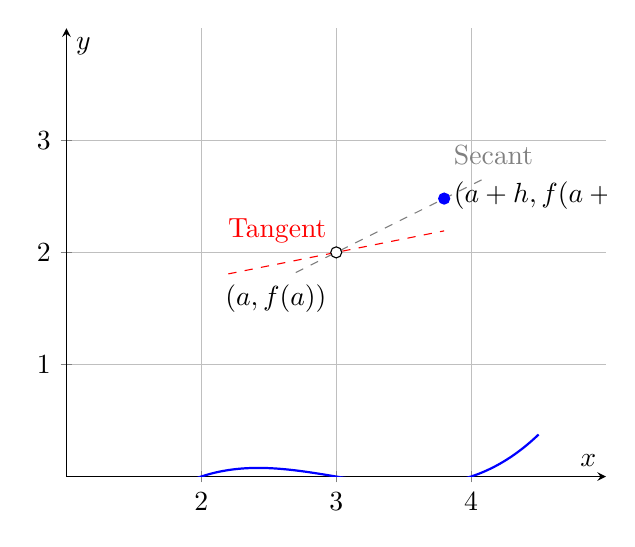
\begin{tikzpicture}

\pgfplotsset{
    soldot/.style={color=blue,only marks,mark=*},
    holdot/.style={color=black,fill=white,only marks,mark=*},
    tangdot/.style={color=red,only marks,mark=*},
    secantline/.style={dashed, color=gray},
    tangentline/.style={dashed, color=red},
    compat=1.12
}
\begin{axis}[
    grid=both,
    axis lines=middle,
    ticklabel style={fill=white},
    xmin=1, xmax=5,
    ymin=0, ymax=4,
    xtick={2, 3, 4},
    ytick={1, 2, 3},
    xlabel=\(x\), ylabel=\(y\),
    samples=200
]
    % The function
    \addplot[domain=1.5:4.5, blue, thick] {0.2*(x^3 - 9*x^2 + 26*x - 24)};

    % Points a and a+h
    \addplot[holdot] coordinates{(3, 2)};
    \addplot[soldot] coordinates{(3.8, 2.48)};
    
    % Labels
    \node at (axis cs:3,1.8) [anchor=north east] {\((a, f(a))\)};
    \node at (axis cs:3.8,2.3) [anchor=south west] {\((a+h, f(a+h))\)};
    
    % Secant line
    \addplot[secantline, domain=2.7:4.1] {0.6*(x - 3) + 2};

    % Tangent line at a
    \addplot[tangentline, domain=2.2:3.8] {0.24*(x - 3) + 2};

    \node[red] at (axis cs:3,2) [anchor=south east] {Tangent};
    \node[gray] at (axis cs:3.8,2.7) [anchor=south west] {Secant};
\end{axis}
  \end{tikzpicture}
  \end{document}
